\documentclass{beamer}

\usepackage[british]{babel}
\usepackage{graphicx,hyperref,ru,url}

% The title of the presentation:
%  - first a short version which is visible at the bottom of each slide;
%  - second the full title shown on the title slide;
\title[RU style for Beamer]{
  Brain Racer}

% Optional: a subtitle to be dispalyed on the title slide


% The author(s) of the presentation:
%  - again first a short version to be displayed at the bottom;
%  - next the full list of authors, which may include contact information;
\author[Stef, Hector, Thomas]{Stef Janssen\\H\'ector van den Boorn\\Thomas van Heyningen }

\begin{document}

\begin{frame}
  \titlepage
\end{frame}

\begin{frame}
  \frametitle{Outline}
  \tableofcontents
\end{frame}

% Section titles are shown in at the top of the slides with the current section 
% highlighted. Note that the number of sections determines the size of the top 
% bar, and hence the university name and logo. If you do not add any sections 
% they will not be visible.


\section{Project}
\begin{frame}
  \frametitle{Problem Description}
\begin{itemize}
 \item Cybathlon: robust zero training classifier
 \item 
\end{itemize}

  \begin{figure}
    \centering
    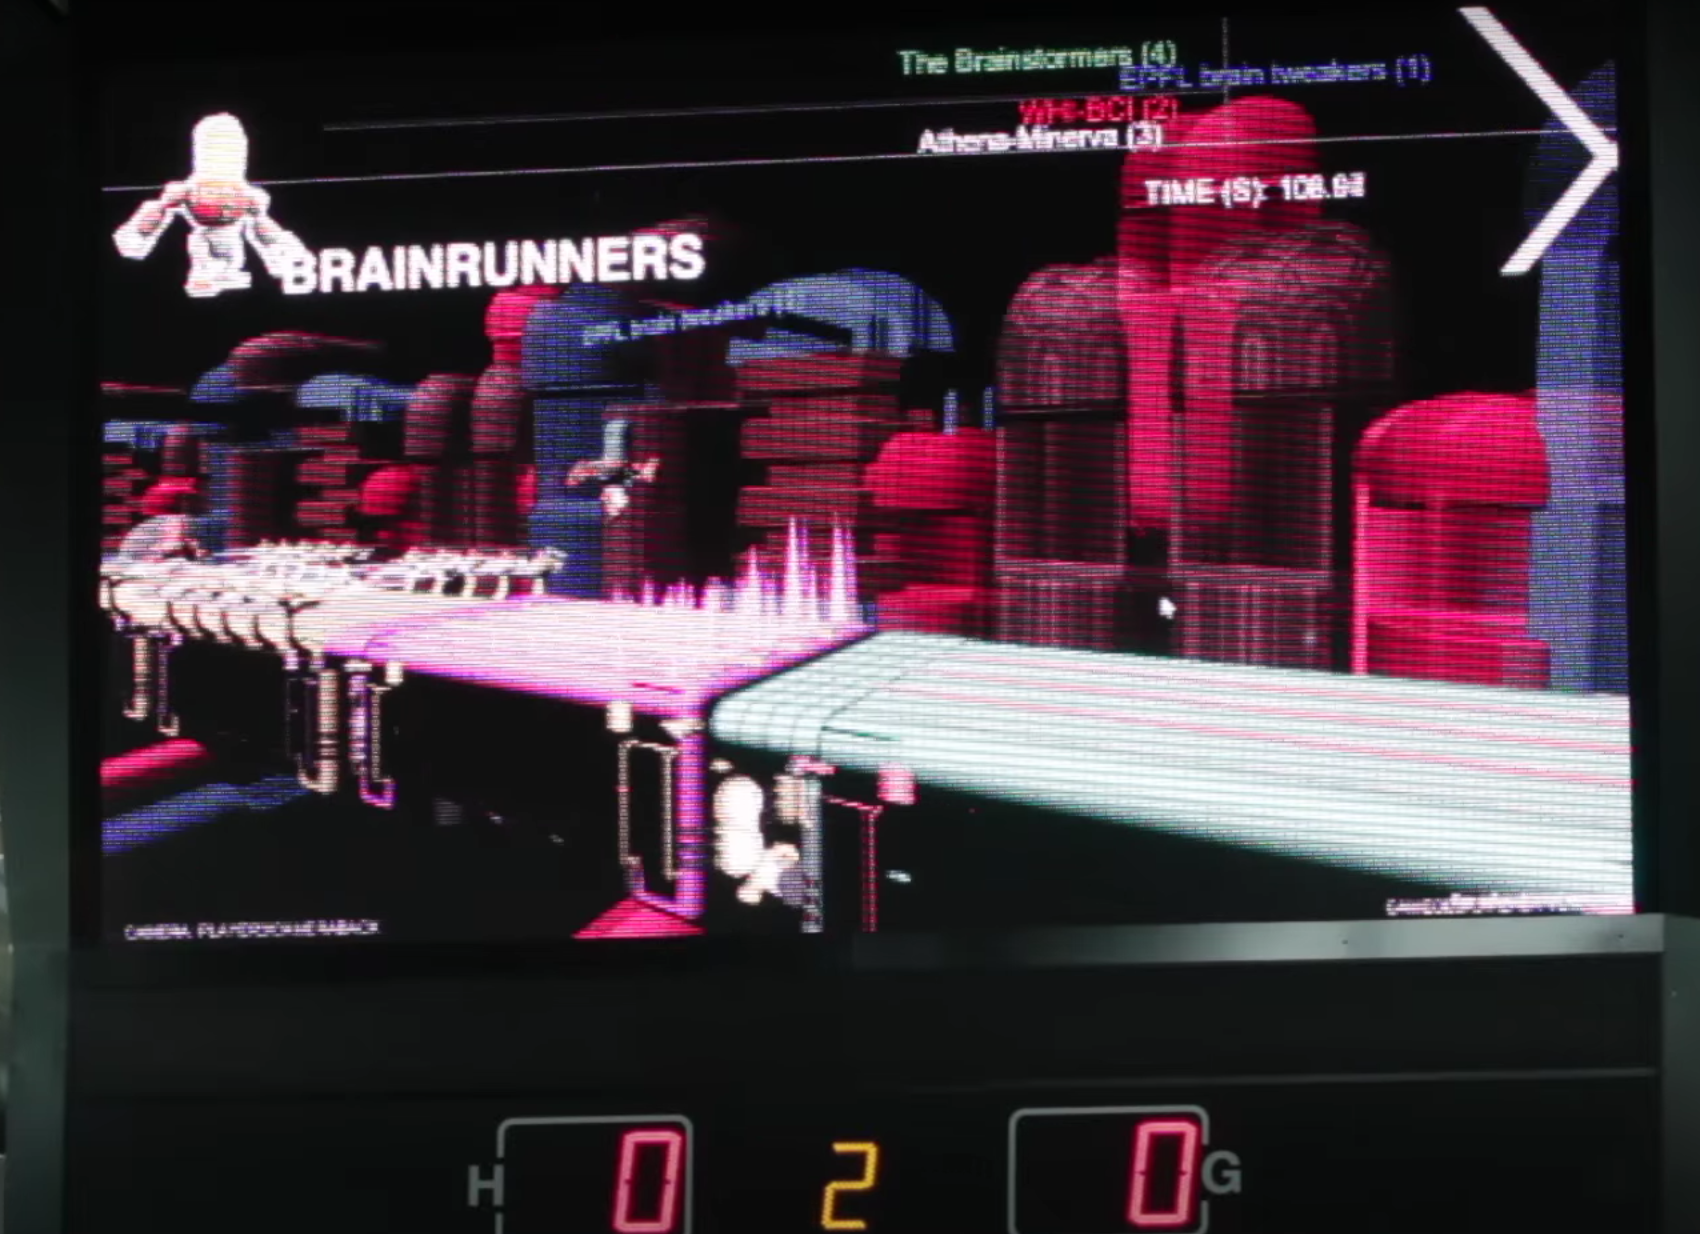
\includegraphics[width=0.4\textwidth]{cybathlon_challenge.png}
  \end{figure}
  
%Ligt toe: simpeler gemaakt naar binaire classificatie
\end{frame}

\begin{frame}
  \frametitle{Foreseen challenges}

  \begin{itemize}
    \item Covariant shift
    \item BCI-performance in general
    \item Generalisability between subjects
    \item more stuff
  \end{itemize}
\end{frame}


\section{Classification scheme}

\begin{frame}
  \frametitle{BCI cycle}
  \begin{figure}
    \centering
    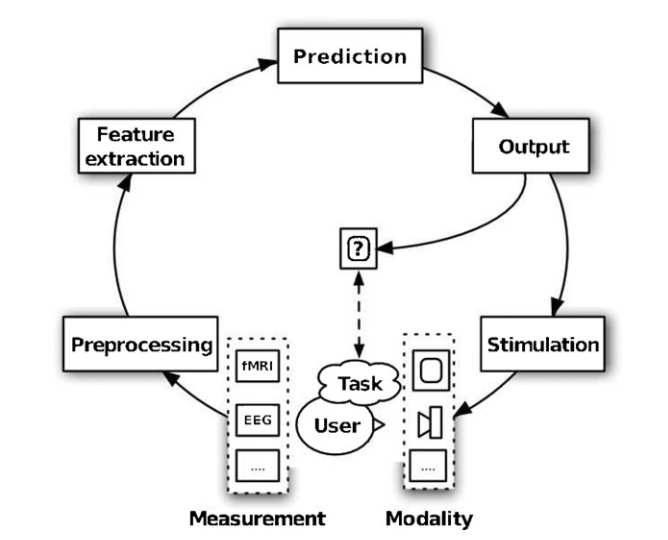
\includegraphics[width=0.7\textwidth]{bci_cycle.png}
  \end{figure}
 
\end{frame}

\begin{frame}
  \frametitle{Preprocessing}

  \begin{itemize}
    \item List all preprocessing
  \end{itemize}
\end{frame}

\begin{frame}
  \frametitle{Feature extraction}
    Fourier transform with large bins
\end{frame}

\begin{frame}
  \frametitle{Prediction}

  \begin{itemize}
    \item List all attempted classifiers
  \end{itemize}
\end{frame}

\begin{frame}
  \frametitle{Stimulation}

  \begin{figure}
    \centering
    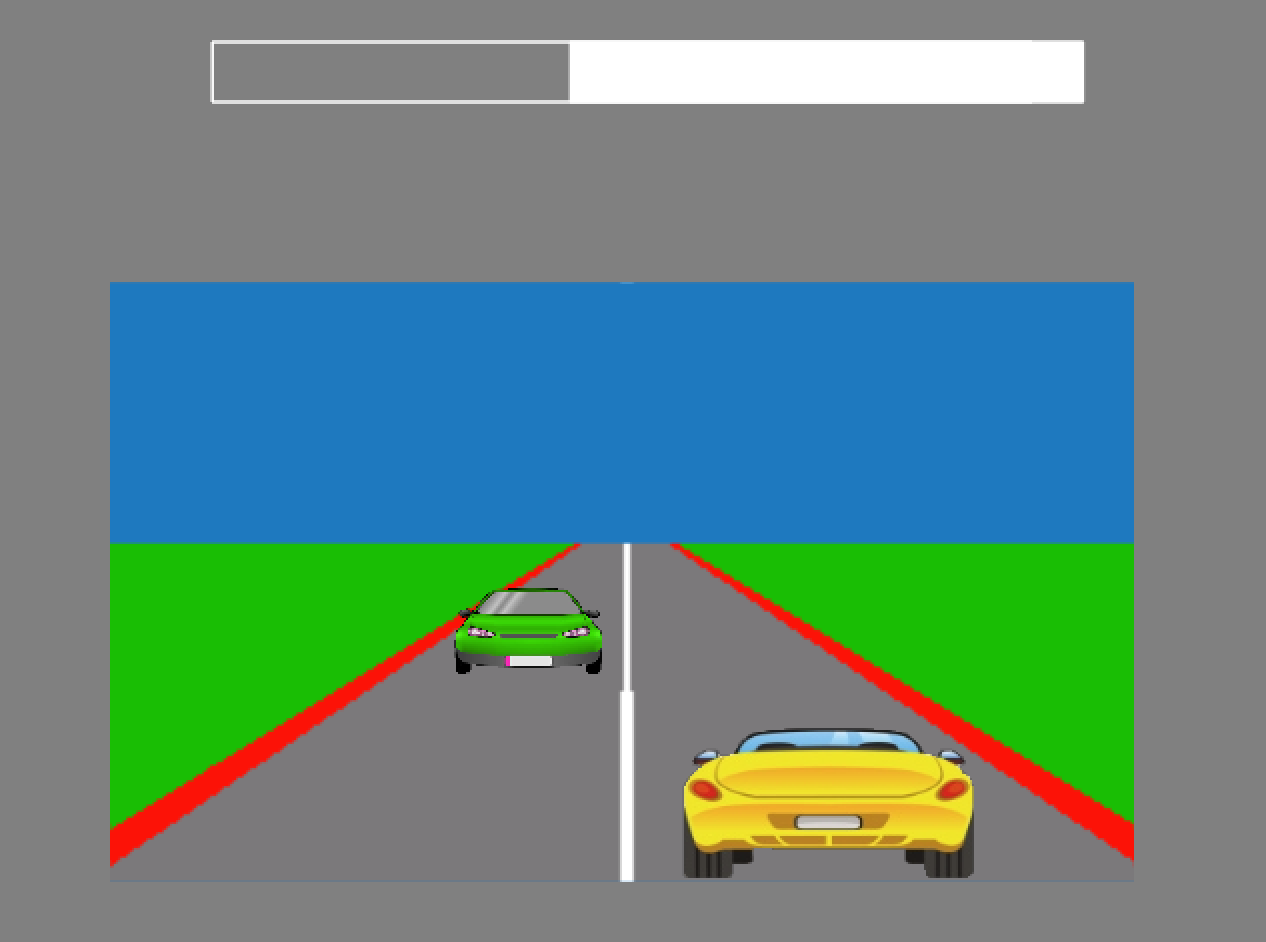
\includegraphics[width=0.7\textwidth]{brain_racer.png}
  \end{figure}
\end{frame}

\section{Experiment pipeline}

\begin{frame}
  \frametitle{Brain racer in Psychopy}

  \begin{figure}
    \centering
    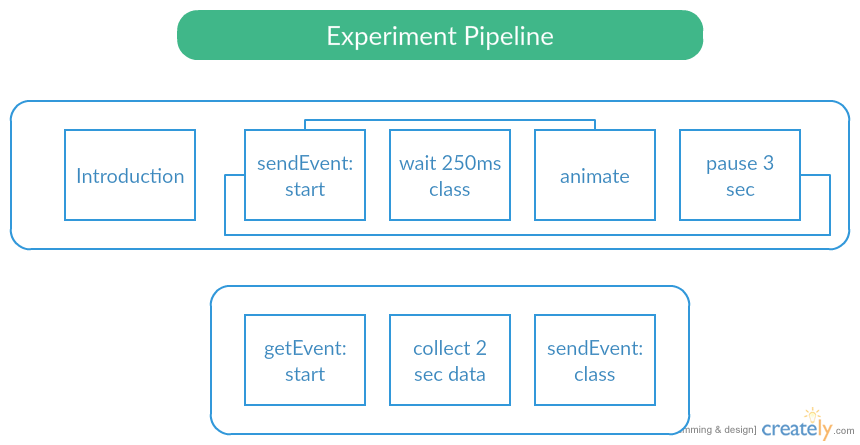
\includegraphics[width=0.9\textwidth]{brain_racer_pipeline.png}
  \end{figure}
\end{frame}

\section{Results}

\begin{frame}

\frametitle{Results}
 \begin{itemize}
   \item Trained on 2 $\rightarrow$ tested on 1
   \item Cross validated on each itself
 \end{itemize}

\end{frame}

\section{Discussion}
\begin{frame}

\frametitle{Discussion}
  \begin{itemize}
   \item Adaptive approach produced sub-optimal results due to the necessity of unsupervised learning
   \item 
  \end{itemize}
\end{frame}



\begin{frame}

\frametitle{Take home message}
The adaptive approach did not work well but decent results were still obtained without training on the specific subject
\end{frame}

\end{document}
